\chapter{Data acquisition and annotation \status{new}}
	\label{chap:data}


    \subsection{Cell culture conditions and imaging modality \status{new}}
    
    rewrite about he type of cells i am tracking briefly, and focus a lot on the imaging technique. Provide examples of different images from different datasets,
    illustrate the problem of out of focus, the out-of-sync shutter, etc.
    
    
    A technique that had crucial impoact on the dientification of the multistep cascade enabling neutrophile recruitmen into inflamed tissues was intrvital microscopy. This method allows the visualization of cells in vivo.
    
    More recently, the introduction of microscopes allowering for thicher tissue penetraction and higher resolution (spinning-disc and two-photon microscopes), more complex tissuea dn organs, sucha as the skin, lives, brain and lung, can also be imaged. The observation of the lung was a challenge for a long time owing to motion artefacts. 
    
    The introbutio of fluorescence (confocal) microscopy  in combination with spinning-disc and two-photon microscopes  has allowed the use of fluorescent antibodies for labelling different cell populations on anatomical structures, as well as the use of transeenic mice with fluorescent leukocyte subsets. 
    
    TODO: I need more data on the different labeled cells (red, green)
    TODO: I need more data on the exact technique and aparatus used to take the images (camera, etc)
    
    \subsection{The annotation tool \statusnew}
    
    	\todo[inline]{some notes on the importance of accurate annotation,s advantages and disadvantages of dot annotations.}
    
    	\todo[inline]{Describe the requirements of an efficient cell annotation tool, such as multipreview, linking, zooming, correct interpretation and saving of the dataformat}
    	
    	\todo[inline]{An overview of the annotation GUI}
    	the multiple displays
    	filter
    	tools for additing/deleting dots and links
    	simultaneous display of detections and links    
    
    \subsection{Annotating cell images \status{new}}
    \rewrite{This describes annotation using Fiji, which was only used at the beginnig}
    What follows is a description of the process of image annotation for use in the machine learning algorithm to detect cells. The image annotation, as required by Arteta's \cite{arteta12} algorithm, are dots on each cell of the image. The algorithm uses these dots as positive examples, and all the remaining pixels as negative examples of a cell.
    
    We have annotated a subset of frames on the Lung dataset provided by Dr. Leo Carlin. The entire dataset is composed of 150 frames, and is divided into two channels, one for each type of cell (\todo{I need to learn more about the types of cells I am tracking}). We have marked 10 cropped frames on each channel (frame 1, 14, 25, 46, 81, 115, 131, 143 and 150) of dimensions about $128\times118$ pixels.
    
    The annotation was performed using a Fiji \cite{fiji12} tool called PointPicker \cite{thevanez14} which is accessible from \(Analyse/Tools/PointPicker\). The annotation is done by manually clicking on each identified cell.The tool outputs a $txt$ file containing $x$ and $y$ coordinates of each annotation, the image number, as well as some other metadata that is not important for us.
    
    \begin{figure}
    	\begin{subfigure}{.49\textwidth}
    	  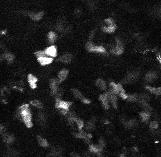
\includegraphics[width=\textwidth]{images/seq_red_crop}
    	\end{subfigure}%
    	\hfill
    	\begin{subfigure}{.49\textwidth}
    	  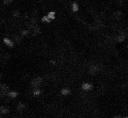
\includegraphics[width=\textwidth]{images/seq_green_crop}
    	\end{subfigure}
    	\caption{Examples of a cropped frame that was annotated for the cell detection machine learning algorithm. Each frame belongs to a different channel of the dataset.}
        \label{fig:annotation_image}
    \end{figure}
    
    It must be noted that the images are very noisy, and it is often hard to distinguish cells from non cells. Figure \ref{fig:annotation_image} displays an example of an image that was annotated. It is therefore questionable how accurately the learning method will be able to learn the idea of a cell, given that the annotations are far from perfect. It would have been much easier to perform the learning using a synthetic dataset.
    
    The data is then loaded into MATLAB and converted into the format required by the algorithm. The data tidying is performed by the script \textit{prepareTrainData.m}.